\section{矩约束下的最小KL}
\label{sec:dsel-min-kl}

上一节的成本是“软”的：成本可以高一点，只要偏离小一点。另一类要求是“硬”的：选出的分布必须满足某些平均量，例如平均点数必须是$10/7$。满足要求的分布在图~\ref{fig:dsel-three-requirements}中排成一条线段，我们要在这条线段上挑出离参考分布最近的一个。

设$\bm{T}:\mathcal{X}\to\mathbb{R}^{k}$可测，$\bm{m}\in\mathbb{R}^{k}$。满足矩要求的分布组成集合
\[
 \mathcal{C}_{\bm{m}}=\Bigl\{Q\in\mathcal{P}(\mathcal{X}):\ \mathbb{E}_{Q}\lVert\bm{T}\rVert_2<\infty,\ \mathbb{E}_{Q}[\bm{T}]=\bm{m}\Bigr\}.
\]
本节研究
\begin{equation}
 \min_{Q\in\mathcal{C}_{\bm{m}}}\ D_{\mathrm{KL}}(Q\Vert P) .
 \label{eq:dsel-min-kl-problem}
\end{equation}
所有能由$P$的绝对连续分布实现的矩组成\term{可行矩集合}（set of feasible moments）
\[
 \mathcal{M}=\Bigl\{\mathbb{E}_{Q}[\bm{T}]:\ Q\ll P,\ \mathbb{E}_{Q}\lVert\bm{T}\rVert_2<\infty\Bigr\}.
\]
只有$\bm{m}\in\mathcal{M}$时问题~\eqref{eq:dsel-min-kl-problem}才有KL有限的候选。

KL的方向在这里是$D_{\mathrm{KL}}(Q\Vert P)$：期望按待选的$Q$计算，有限的前提是$Q\ll P$。所以选出的分布可以删去$P$的某些状态，却不会在$P$认为不可能的地方放质量。参考分布代表原有的认识，矩要求是新加的条件，问题问的是：为了满足新条件，最少要把原有认识改动多少。若反过来最小化$D_{\mathrm{KL}}(P\Vert Q)$，期望按$P$计算，要求$Q$覆盖$P$的全部状态，这对应另一类问题，在第~\ref{chap:distribution-approximation}章讨论。

\subsection{指数倾斜}
\label{sec:dsel-tilt}

先在有限状态上求解。设$\mathcal{X}$有限，$p(x)>0$对每个$x$成立。这时每个$Q$都绝对连续于$P$，$Q$的矩是$\bm{T}(x)$的凸组合，而任何凸组合也都能由某个$Q$实现，所以
\[
 \mathcal{M}=\operatorname{conv}\{\bm{T}(x):x\in\mathcal{X}\}
\]
是有限个点的凸包。在例子中$T(x)=x$，$\mathcal{M}=[0,2]$。

\paragraph{乘子方程}
在概率三角形内部形式地求驻点。对归一化引入乘子$\nu$，对矩约束引入乘子向量$\bm{\theta}\in\mathbb{R}^{k}$，Lagrange函数为
\[
 \sum_xq(x)\ln\frac{q(x)}{p(x)}-\Bigl\langle\bm{\theta},\sum_xq(x)\bm{T}(x)-\bm{m}\Bigr\rangle-\nu\Bigl(\sum_xq(x)-1\Bigr).
\]
对$q(x)$求偏导并令其为零，得到
\[
 \ln\frac{q(x)}{p(x)}+1-\langle\bm{\theta},\bm{T}(x)\rangle-\nu=0 .
\]

解出
\[
 q(x)=p(x)\exp\bigl(\langle\bm{\theta},\bm{T}(x)\rangle\bigr)\,\mathrm{e}^{\nu-1} ,
\]
再由归一化定出常数因子：
\begin{equation}
 q_{\bm{\theta}}(x)=p(x)\exp\bigl(\langle\bm{\theta},\bm{T}(x)\rangle-A(\bm{\theta})\bigr),\qquad A(\bm{\theta})=\ln\sum_xp(x)\,\mathrm{e}^{\langle\bm{\theta},\bm{T}(x)\rangle} .
 \label{eq:dsel-tilt-finite}
\end{equation}
乘子$\bm{\theta}$还没有确定，它要使$q_{\bm{\theta}}$满足矩约束。Lagrange乘子法给出的是必要条件的形式（见\BookChapterRef{chap:constrained-optimality}{卷五第17章“约束问题的最优性”}），这里又假设了解在内部，所以式~\eqref{eq:dsel-tilt-finite}仍只是候选。

这个形式在一般空间上同样有意义。

\begin{definition}[指数倾斜]
\label{def:dsel-tilt}
设$P\in\mathcal{P}(\mathcal{X})$，$\bm{\theta}\in\mathbb{R}^{k}$，并且
\begin{equation}
 A(\bm{\theta})=\ln\mathbb{E}_{P}\bigl[\mathrm{e}^{\langle\bm{\theta},\bm{T}\rangle}\bigr]<\infty .
 \label{eq:dsel-tilt-partition}
\end{equation}
以
\begin{equation}
 \frac{\mathrm{d}Q_{\bm{\theta}}}{\mathrm{d}P}=\exp\bigl(\langle\bm{\theta},\bm{T}\rangle-A(\bm{\theta})\bigr)
 \label{eq:dsel-tilt}
\end{equation}
定义的$Q_{\bm{\theta}}$称为$P$沿$\bm{T}$的\term{指数倾斜}（exponential tilting）。
\end{definition}

全体$Q_{\bm{\theta}}$就是第~\ref{chap:distribution-families}章以$P$为基准测度、以$\bm{T}$为自然统计量的指数族，$A$是它的对数配分函数。密度处处为正，所以每个$Q_{\bm{\theta}}$与$P$互相绝对连续。在例子中，$P$均匀，$T(x)=x$，$q_\theta(x)\propto\mathrm{e}^{\theta x}$。取$\theta=\ln2$，三个权重是$1,2,4$，
\[
 Q_{\ln2}=\Bigl(\frac17,\ \frac27,\ \frac47\Bigr),\qquad\mathbb{E}_{Q_{\ln2}}[X]=\frac{2+8}{7}=\frac{10}{7},
\]
它恰好落在约束线段上。

\paragraph{勾股恒等式}
要说明$Q_{\ln2}$比线段上其他分布更接近$P$，不必求导，只需把$D_{\mathrm{KL}}(Q\Vert P)$拆开，得到下面的\term{勾股恒等式}。

\begin{lemma}[勾股恒等式]
\label{lem:dsel-pythagoras}
设$A(\bm{\theta})<\infty$，$Q\in\mathcal{C}_{\bm{m}}$且$D_{\mathrm{KL}}(Q\Vert P)<\infty$。则
\begin{equation}
 D_{\mathrm{KL}}(Q\Vert P)=D_{\mathrm{KL}}(Q\Vert Q_{\bm{\theta}})+\langle\bm{\theta},\bm{m}\rangle-A(\bm{\theta}) .
 \label{eq:dsel-pythagoras-general}
\end{equation}
若$Q_{\bm{\theta}}$本身也属于$\mathcal{C}_{\bm{m}}$，则
\begin{equation}
 D_{\mathrm{KL}}(Q\Vert P)=D_{\mathrm{KL}}(Q\Vert Q_{\bm{\theta}})+D_{\mathrm{KL}}(Q_{\bm{\theta}}\Vert P) .
 \label{eq:dsel-pythagoras}
\end{equation}
\end{lemma}

\begin{proof}
$Q\ll P$，而$P$与$Q_{\bm{\theta}}$互相绝对连续，所以$Q\ll Q_{\bm{\theta}}$。由链式法则与式~\eqref{eq:dsel-tilt}，
\[
 \ln\frac{\mathrm{d}Q}{\mathrm{d}Q_{\bm{\theta}}}=\ln\frac{\mathrm{d}Q}{\mathrm{d}P}-\langle\bm{\theta},\bm{T}\rangle+A(\bm{\theta}) .
\]
右边第一项在$Q$下可积（KL有限，负部总可积），第二项因$\mathbb{E}_{Q}\lVert\bm{T}\rVert_2<\infty$可积。逐项取$Q$下的期望，并用$\mathbb{E}_{Q}[\bm{T}]=\bm{m}$，
\[
 D_{\mathrm{KL}}(Q\Vert Q_{\bm{\theta}})=D_{\mathrm{KL}}(Q\Vert P)-\langle\bm{\theta},\bm{m}\rangle+A(\bm{\theta}) ,
\]
移项即得式~\eqref{eq:dsel-pythagoras-general}。若$Q_{\bm{\theta}}\in\mathcal{C}_{\bm{m}}$，则式~\eqref{eq:dsel-tilt}给出的对数密度在$Q_{\bm{\theta}}$下可积，其期望是
\[
 D_{\mathrm{KL}}(Q_{\bm{\theta}}\Vert P)=\langle\bm{\theta},\bm{m}\rangle-A(\bm{\theta}) .
\]
代回式~\eqref{eq:dsel-pythagoras-general}即得式~\eqref{eq:dsel-pythagoras}。
\end{proof}

证明的关键一步是：$\ln(\mathrm{d}Q_{\bm{\theta}}/\mathrm{d}P)$只通过$\bm{T}$依赖于$x$，而约束集合中所有分布的$\bm{T}$平均值都相同，所以这个对数比在约束集合上的平均是常数。

在例子中验证。取线段的一个端点$Q=(\tfrac27,0,\tfrac57)$，三个散度分别是
\[
 \begin{gathered}
 D_{\mathrm{KL}}(Q\Vert P)=\tfrac27\ln\tfrac67+\tfrac57\ln\tfrac{15}7\approx0.5003,\\
 D_{\mathrm{KL}}(Q\Vert Q_{\ln2})=\tfrac27\ln2+\tfrac57\ln\tfrac54\approx0.3574,\qquad D_{\mathrm{KL}}(Q_{\ln2}\Vert P)\approx0.1429 .
 \end{gathered}
\]
后两项之和正是第一项。图~\ref{fig:dsel-pythagoras}把这三个量画成一个“直角三角形”：约束集合是一条直线，倾斜族是与它相交的曲线，交点$Q_{\ln2}$像是垂足。

\begin{BookInlineFigure}
 \centering
 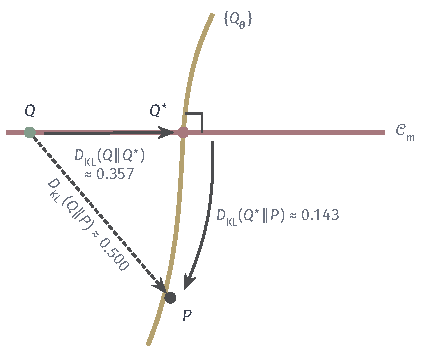
\includegraphics[width=72mm]{figures/07-probability/07-distribution-optimization/tikz/dsel-pythagoras/figure.pdf}
 \caption{勾股恒等式的示意。红线是约束集合$\mathcal{C}_{\bm{m}}$，黄线是倾斜族$\{Q_{\bm{\theta}}\}$，两者交于$Q^{*}=Q_{\ln2}$。箭头从KL的第一个分布指向第二个分布，数值取自$P$均匀、$T(x)=x$、$m=10/7$、$Q=(\frac27,0,\frac57)$的例子，单位为nat。}
 \label{fig:dsel-pythagoras}
\end{BookInlineFigure}

这个“勾股”只是类比。KL散度不对称，也不满足三角不等式，恒等式~\eqref{eq:dsel-pythagoras}只在一个点位于约束集合、另一个点是满足同一约束的倾斜分布时成立。三角形中实际的几何如图~\ref{fig:dsel-kl-projection}：以$P$为中心的KL等值线一圈圈向外扩张，第一次碰到约束线段的地方就是$Q_{\ln2}$，倾斜族的曲线恰好从这一点穿过。

\begin{BookInlineFigure}
 \centering
 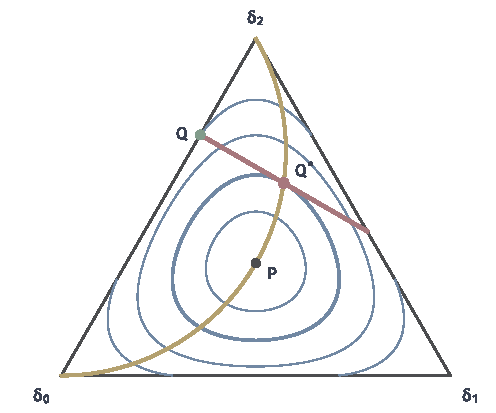
\includegraphics[width=84mm]{figures/07-probability/07-distribution-optimization/matplotlib/dsel-kl-projection/figure.pdf}
 \caption{约束线段上离$P$最近的分布。蓝线是$D_{\mathrm{KL}}(Q\Vert P)$的等值线，取值$0.05,0.3,0.5$（细）与最小值$D^{*}\approx0.1429$（粗）；红色线段是$\mathbb{E}_{Q}[X]=10/7$；黄线是倾斜族$q_\theta\propto\mathrm{e}^{\theta x}$。粗等值线在红点$Q^{*}=(\frac17,\frac27,\frac47)$处与线段相切；绿点$Q=(\frac27,0,\frac57)$满足约束，但落在更外圈。}
 \label{fig:dsel-kl-projection}
\end{BookInlineFigure}

\paragraph{最优性与存在性}
引理把最优性归结为一件事：能否找到$\bm{\theta}$，使$Q_{\bm{\theta}}$满足约束。这需要$\bm{m}$离可行矩集合的边界有一段距离。可行矩集合可能是低维的，例如当所有$\bm{T}(x)$都落在$\mathbb{R}^{2}$的一条直线上时，$\mathcal{M}$是一条线段，它在平面中没有内点。所以“远离边界”要在$\mathcal{M}$所在的仿射包$\operatorname{aff}\mathcal{M}$内衡量：$\bm{m}$属于$\mathcal{M}$的相对内部$\operatorname{ri}\mathcal{M}$，是指存在$\varepsilon>0$，使$\operatorname{aff}\mathcal{M}$中与$\bm{m}$距离小于$\varepsilon$的点都在$\mathcal{M}$中。上面的线段，相对内部就是去掉两个端点。

\begin{theorem}[指数倾斜给出最小KL]
\label{thm:dsel-min-kl}
设$\mathcal{X}$有限，$p(x)>0$对每个$x$成立，$\bm{m}\in\operatorname{ri}\mathcal{M}$。则
\begin{enumerate}
 \item 存在$\bm{\theta}^{*}\in\mathbb{R}^{k}$，使$\mathbb{E}_{Q_{\bm{\theta}^{*}}}[\bm{T}]=\bm{m}$；
 \item $Q^{*}=Q_{\bm{\theta}^{*}}$是问题~\eqref{eq:dsel-min-kl-problem}的唯一最优分布，最优值为
 \begin{equation}
 D^{*}=\langle\bm{\theta}^{*},\bm{m}\rangle-A(\bm{\theta}^{*}) ;
 \label{eq:dsel-min-kl-value}
 \end{equation}
 \item 满足第一条的$\bm{\theta}^{*}$可能不唯一，但它们给出同一个$Q^{*}$。
\end{enumerate}
\end{theorem}

\begin{proof}
第一部分。令
\[
 \ell(\bm{\theta})=\langle\bm{\theta},\bm{m}\rangle-A(\bm{\theta}) ,
\]
我们证明它有最大值点，并且最大值点满足矩约束。把$\ell$写成
\[
 -\ell(\bm{\theta})=\ln\sum_xp(x)\,\mathrm{e}^{\langle\bm{\theta},\bm{T}(x)-\bm{m}\rangle} .
\]
记
\[
 L=\operatorname{span}\{\bm{T}(x)-\bm{m}:x\in\mathcal{X}\} .
\]
因为$\bm{m}\in\mathcal{M}$，有$\operatorname{aff}\mathcal{M}=\bm{m}+L$。若$\bm{a}\perp L$，则每个指数中$\langle\bm{a},\bm{T}(x)-\bm{m}\rangle=0$，所以$\ell(\bm{\theta}+\bm{a})=\ell(\bm{\theta})$。只需在子空间$L$上找最大值点。

对$L$中的单位向量$\bm{u}$，令
\[
 \delta(\bm{u})=\max_{x\in\mathcal{X}}\langle\bm{u},\bm{T}(x)-\bm{m}\rangle .
\]
由于$\bm{m}\in\operatorname{ri}\mathcal{M}$，存在$\varepsilon>0$使$\bm{m}+\varepsilon\bm{u}\in\mathcal{M}$，即它是某个凸组合$\sum_xq(x)\bm{T}(x)$。与$\bm{u}$作内积，
\[
 \varepsilon=\sum_xq(x)\langle\bm{u},\bm{T}(x)-\bm{m}\rangle\leq\delta(\bm{u}) .
\]
所以$\delta(\bm{u})>0$。$\delta$在$L$的单位球面上连续，球面紧，于是$\delta_0=\min\delta(\bm{u})>0$。

对$\bm{\theta}\in L$，$\bm{\theta}\neq\bm{0}$，取$\bm{u}=\bm{\theta}/\lVert\bm{\theta}\rVert_2$。和式中至少有一项的指数是$\lVert\bm{\theta}\rVert_2\,\delta(\bm{u})$，其余各项为正，记$p_{\min}=\min_xp(x)>0$，得到
\[
 -\ell(\bm{\theta})\geq\ln p_{\min}+\delta_0\lVert\bm{\theta}\rVert_2 .
\]
所以$-\ell$在$L$上连续且当$\lVert\bm{\theta}\rVert_2\to\infty$时趋于$+\infty$，它在$L$的某个闭球上取到在$L$上的最小值，设最小值点为$\bm{\theta}^{*}$。由$\ell$沿$L^{\perp}$不变，$\bm{\theta}^{*}$也是$\ell$在整个$\mathbb{R}^{k}$上的最大值点。

$\ell$可微，最大值点处梯度为零。对式~\eqref{eq:dsel-tilt-finite}中的$A$求梯度，
\[
 \nabla A(\bm{\theta})=\frac{\sum_xp(x)\bm{T}(x)\mathrm{e}^{\langle\bm{\theta},\bm{T}(x)\rangle}}{\sum_xp(x)\mathrm{e}^{\langle\bm{\theta},\bm{T}(x)\rangle}}=\mathbb{E}_{Q_{\bm{\theta}}}[\bm{T}] .
\]
于是
\[
 \nabla\ell(\bm{\theta}^{*})=\bm{m}-\mathbb{E}_{Q_{\bm{\theta}^{*}}}[\bm{T}]=\bm{0} .
\]


第二部分。有限状态上每个$Q\in\mathcal{C}_{\bm{m}}$都满足$D_{\mathrm{KL}}(Q\Vert P)<\infty$。由引理~\ref{lem:dsel-pythagoras}，
\[
 D_{\mathrm{KL}}(Q\Vert P)=D_{\mathrm{KL}}(Q\Vert Q^{*})+D_{\mathrm{KL}}(Q^{*}\Vert P)\geq D_{\mathrm{KL}}(Q^{*}\Vert P),
\]
等号当且仅当$D_{\mathrm{KL}}(Q\Vert Q^{*})=0$，即$Q=Q^{*}$。最优值由引理中的表达式给出。

第三部分。若$\bm{\theta}^{*}$与$\bm{\theta}'$都满足矩约束，则$Q_{\bm{\theta}^{*}}$与$Q_{\bm{\theta}'}$都是最优分布，由唯一性二者相同。
\end{proof}

三个条件各有作用。$p(x)>0$保证每个候选都绝对连续于$P$；若$P$有零概率的状态，先把它们从$\mathcal{X}$中删去即可。有限性保证$A(\bm{\theta})$对一切$\bm{\theta}$有限，也提供了证明中的紧性。$\bm{m}\in\operatorname{ri}\mathcal{M}$保证存在有限的$\bm{\theta}^{*}$；第~\ref{sec:dsel-moment-matching}节会看到，$\bm{m}$在边界上时最优分布仍然存在，但不再是任何$Q_{\bm{\theta}}$。

在例子中，$\theta^{*}=\ln2$，$A(\ln2)=\ln\frac{1+2+4}{3}=\ln\frac73$，由式~\eqref{eq:dsel-min-kl-value}，
\[
 D^{*}=\frac{10}{7}\ln2-\ln\frac73\approx0.9902-0.8473=0.1429 ,
\]
与直接计算一致。

\paragraph{指数族从哪里来}
问题~\eqref{eq:dsel-min-kl-problem}的候选是$\mathcal{X}$上的全部分布，并没有限定在某个参数族中，最优解却落在以$P$为基准、以约束统计量$\bm{T}$为自然统计量的指数族里。Lagrange乘子变成了自然参数，要约束哪些平均量，就决定了用哪些统计量作指数权重。所以这一步不能理解为“先选一个指数族，再在族内近似”：族是最优性条件的产物。第~\ref{chap:distribution-approximation}章研究的是另一类问题，那里先限定候选族，再在族内逼近一个给定的目标分布。

上一节的Gibbs分布也是这样的解。取$\bm{T}=V$，$\bm{\theta}=-1/\tau$，Gibbs分布$Q^{*}_\tau$就是$P$沿$V$的倾斜；由定理~\ref{thm:dsel-min-kl}，它是所有满足$\mathbb{E}_{Q}[V]=\mathbb{E}_{Q^{*}_\tau}[V]$的分布中离$P$最近的一个。例如$(\tfrac47,\tfrac27,\tfrac17)$是平均成本为$4/7$的分布中KL最小者。成本加罚的软约束与矩的硬约束，在指数倾斜这里汇合。

\subsection{矩匹配}
\label{sec:dsel-moment-matching}

定理~\ref{thm:dsel-min-kl}把“选一个分布”变成了“解一个方程”：找$\bm{\theta}$使
\begin{equation}
 \nabla A(\bm{\theta})=\mathbb{E}_{Q_{\bm{\theta}}}[\bm{T}]=\bm{m} .
 \label{eq:dsel-moment-matching}
\end{equation}
这称为\term{矩匹配方程}（moment-matching equation）。未知数只有$k$个，与$\mathcal{X}$的大小无关。第~\ref{chap:distribution-families}章已经知道，在自然参数域内部$\nabla A$是均值映射，$A$的Hessian是统计量的协方差矩阵：
\[
 \nabla^{2}A(\bm{\theta})=\operatorname{Cov}_{Q_{\bm{\theta}}}(\bm{T}) .
\]
本小节用这两个事实分析方程的求解、冗余统计量的影响和边界上的矩。

\paragraph{对偶函数}
式~\eqref{eq:dsel-pythagoras-general}还给出一个与$\bm{\theta}$是否满足约束无关的不等式。由$D_{\mathrm{KL}}(Q\Vert Q_{\bm{\theta}})\geq0$，对每个$Q\in\mathcal{C}_{\bm{m}}$与每个使$A(\bm{\theta})$有限的$\bm{\theta}$，
\begin{equation}
 D_{\mathrm{KL}}(Q\Vert P)\geq\ell(\bm{\theta})=\langle\bm{\theta},\bm{m}\rangle-A(\bm{\theta}) .
 \label{eq:dsel-weak-duality}
\end{equation}
这个不等式不要求$\mathcal{X}$有限。每个$\bm{\theta}$给出最优值的一个下界，每个可行的$Q$给出一个上界。$\ell$称为对偶函数，它是凹函数，因为$A$是凸函数。

方程~\eqref{eq:dsel-moment-matching}正是$\nabla\ell(\bm{\theta})=\bm{0}$，即$\bm{\theta}$是$\ell$的最大值点。在定理~\ref{thm:dsel-min-kl}的条件下，上下界在这里相遇：
\[
 \max_{\bm{\theta}}\ell(\bm{\theta})=\min_{Q\in\mathcal{C}_{\bm{m}}}D_{\mathrm{KL}}(Q\Vert P) .
\]
这就是Lagrange对偶，下界~\eqref{eq:dsel-weak-duality}是弱对偶，等号是强对偶（一般理论见\BookChapterRef{chap:duality}{卷五第18章“对偶问题”}）。$k$维的凹函数最大化比在全体分布上的最小化容易得多，这是实际求解时总是转到$\bm{\theta}$上的原因。

图~\ref{fig:dsel-dual-function}画出例子中的$-\ell(\theta)=A(\theta)-\theta m$。$m=1$时最小值点是$\theta=0$，因为$P$本身已满足约束，$D^{*}=0$。$m=10/7$时最小值点是$\ln2$，最小值$-D^{*}\approx-0.1429$。$m=2$在可行矩集合$[0,2]$的端点，曲线单调下降，趋于$-\ln3$而达不到：上界与下界仍相等，因为唯一可行的分布$\delta_2$满足$D_{\mathrm{KL}}(\delta_2\Vert P)=\ln3$，但没有有限的$\theta$达到它。

\begin{BookInlineFigure}
 \centering
 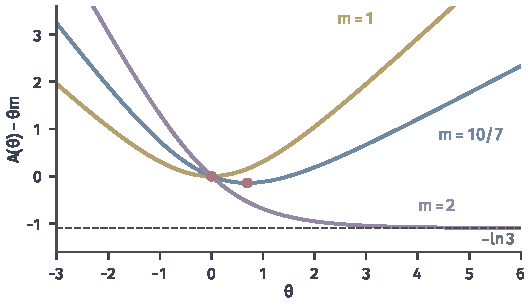
\includegraphics[width=90mm]{figures/07-probability/07-distribution-optimization/matplotlib/dsel-dual-function/figure.pdf}
 \caption{对偶函数取负号后的$A(\theta)-\theta m$，$A(\theta)=\ln\frac{1+\mathrm{e}^{\theta}+\mathrm{e}^{2\theta}}{3}$。黄：$m=1$，最小值$0$在$\theta=0$；蓝：$m=10/7$，最小值$-0.1429$在$\theta=\ln2$（红点）；紫：$m=2$，单调下降，下确界$-\ln3$（深灰虚线）不被达到。}
 \label{fig:dsel-dual-function}
\end{BookInlineFigure}

\paragraph{Hessian与局部求解}
对偶函数的Hessian是协方差矩阵的相反数。对任意$\bm{a}$，
\[
 \bm{a}^{\top}\operatorname{Cov}_{Q_{\bm{\theta}}}(\bm{T})\,\bm{a}=\operatorname{Var}_{Q_{\bm{\theta}}}\bigl(\langle\bm{a},\bm{T}\rangle\bigr)\geq0 ,
\]
等号当且仅当$\langle\bm{a},\bm{T}\rangle$在$Q_{\bm{\theta}}$下几乎必然为常数。有限状态、$p>0$时$Q_{\bm{\theta}}$处处为正，这就是$\langle\bm{a},\bm{T}(x)\rangle$对所有$x$相等。若不存在这样的$\bm{a}\neq\bm{0}$，即统计量之间没有仿射关系，则协方差矩阵对每个$\bm{\theta}$正定。

协方差正定时，$\bm{\theta}\mapsto\nabla A(\bm{\theta})$的Jacobian矩阵可逆，由反函数定理（见\BookChapterRef{chap:implicit-inverse-functions}{卷二第22章“隐函数与反函数”}），它的逆$\bm{m}\mapsto\bm{\theta}(\bm{m})$在$\operatorname{ri}\mathcal{M}$上光滑，导数是协方差矩阵的逆：
\[
 \frac{\partial\bm{\theta}}{\partial\bm{m}}=\operatorname{Cov}_{Q_{\bm{\theta}}}(\bm{T})^{-1} .
\]
在例子中$m=10/7$处$\operatorname{Var}_{Q_{\ln2}}(X)=26/49$，所以$\mathrm{d}\theta/\mathrm{d}m=49/26\approx1.885$：平均值再提高$0.01$，参数约需增加$0.019$。方差越小，同样的矩变化需要越大的参数变化；靠近可行矩集合的边界时方差趋于零，参数随之发散，这在后面的边界情形中会看到。

求解方程~\eqref{eq:dsel-moment-matching}的标准方法是Newton法：在当前点把$\nabla A$线性化，令线性化后的矩等于$\bm{m}$。迭代公式是
\begin{equation}
 \bm{\theta}^{(t+1)}=\bm{\theta}^{(t)}-\operatorname{Cov}_{Q_{\bm{\theta}^{(t)}}}(\bm{T})^{-1}\Bigl(\mathbb{E}_{Q_{\bm{\theta}^{(t)}}}[\bm{T}]-\bm{m}\Bigr).
 \label{eq:dsel-newton}
\end{equation}
它也是对凹函数$\ell$的Newton法（见\BookChapterRef{chap:second-order-methods}{卷五第7章“二阶方法”}）。每一步需要在当前倾斜分布下计算$\bm{T}$的均值与协方差。

在例子中从$\theta^{(0)}=0$出发。此时$Q$均匀，均值$1$，方差$2/3$，由式~\eqref{eq:dsel-newton}，
\[
 \theta^{(1)}=0-\frac{1-10/7}{2/3}=\frac{9}{14}\approx0.6429 .
\]
在$\theta^{(1)}$处，$Q\approx(0.1534,0.2917,0.5549)$，均值约$1.40147$，方差约$0.54708$，于是
\[
 \theta^{(2)}\approx0.6429-\frac{1.40147-1.42857}{0.54708}\approx0.692394 .
\]
再一步得到$\theta^{(3)}\approx0.6931470$，与$\ln2=0.69314718\ldots$相差约$2\times10^{-7}$。矩残差依次约为$0.43$、$2.7\times10^{-2}$、$4.0\times10^{-4}$、$9.4\times10^{-8}$，每步有效数字约翻倍，这是Newton法在解附近的二次收敛。

离解较远时，线性化可能越过头。图~\ref{fig:dsel-newton-steps}(a)从$\theta^{(0)}=-1$出发，第一步跳到$1.365$，越过了$\ln2$，第二步回到$0.451$，之后才进入二次收敛的范围。因为$\ell$是凹的，加上沿Newton方向的步长搜索即可保证从任意起点收敛；协方差接近奇异时，步长与方程的病态都要另作处理。

\begin{BookInlineFigure}
 \centering
 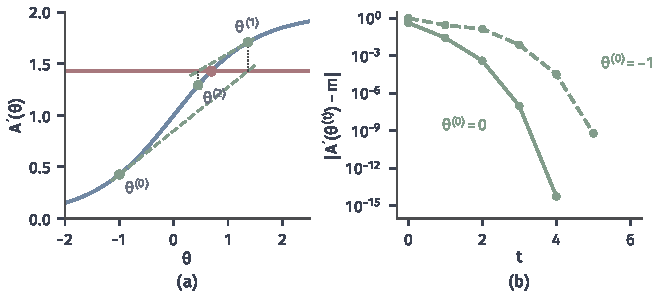
\includegraphics[width=112mm]{figures/07-probability/07-distribution-optimization/matplotlib/dsel-newton-steps/figure.pdf}
 \caption{用Newton法解矩匹配方程$A'(\theta)=10/7$。(a)均值映射$A'(\theta)$（蓝），目标水平$m=10/7$（红线），从$\theta^{(0)}=-1$出发的前两条切线（绿色虚线）与迭代点（绿）；红点是解$\theta=\ln2$。(b)矩残差$\lvert A'(\theta^{(t)})-m\rvert$，纵轴为对数刻度，实线从$\theta^{(0)}=0$出发，虚线从$\theta^{(0)}=-1$出发。}
 \label{fig:dsel-newton-steps}
\end{BookInlineFigure}

\paragraph{冗余统计量}
若统计量之间有仿射关系，协方差矩阵就奇异，Newton步中的线性方程不能唯一求解。取$\bm{T}(x)=(x,\,2-x)$，要求$\bm{m}=(\tfrac{10}7,\tfrac47)$。两个约束说的是同一件事，因为$T_1+T_2\equiv2$。倾斜分布为
\[
 q_{\bm{\theta}}(x)\propto\mathrm{e}^{\theta_1x+\theta_2(2-x)}=\mathrm{e}^{2\theta_2}\,\mathrm{e}^{(\theta_1-\theta_2)x},
\]
只依赖$\theta_1-\theta_2$。满足矩约束的$\bm{\theta}$组成整条直线$\theta_1-\theta_2=\ln2$，它们给出同一个$Q^{*}=(\tfrac17,\tfrac27,\tfrac47)$，正如定理~\ref{thm:dsel-min-kl}第三部分所说。记$v=\operatorname{Var}_{Q_{\bm{\theta}}}(X)$，协方差矩阵
\[
 \operatorname{Cov}_{Q_{\bm{\theta}}}(\bm{T})=v\begin{bmatrix}1&-1\\-1&1\end{bmatrix}
\]
沿$(1,1)$方向为零。图~\ref{fig:dsel-redundant}中，对偶函数的等值线都平行于$(1,1)$，最大值点不是一个点而是一条谷线。

\begin{BookInlineFigure}
 \centering
 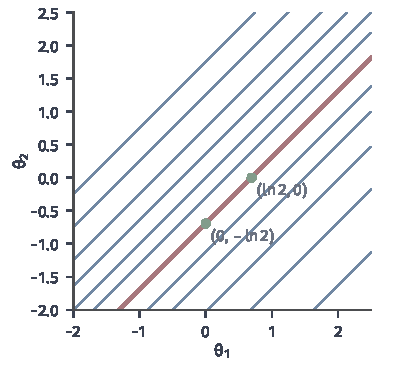
\includegraphics[width=70mm]{figures/07-probability/07-distribution-optimization/matplotlib/dsel-redundant/figure.pdf}
 \caption{冗余统计量$\bm{T}(x)=(x,2-x)$时的对偶函数，$P$均匀，$\bm{m}=(\frac{10}7,\frac47)$。蓝线是$A(\bm{\theta})-\langle\bm{\theta},\bm{m}\rangle$的等值线，全部平行于$(1,1)$；红线$\theta_1-\theta_2=\ln2$上每一点都是最优参数，绿点$(0,-\ln2)$与$(\ln2,0)$是其中两个，它们给出同一个分布。}
 \label{fig:dsel-redundant}
\end{BookInlineFigure}

处理办法有两种：删去多余的统计量，使表示成为第~\ref{chap:distribution-families}章的最小表示；或者保留冗余，在奇异的线性方程中取任意一个解，例如范数最小的解，最后得到的分布不受影响。冗余还带来一个必须先检查的问题：矩要求本身要相容。若要求$\bm{m}=(\tfrac{10}7,1)$，则$m_1+m_2\neq2$，$\bm{m}$不在$\operatorname{aff}\mathcal{M}$中，没有任何分布满足它；这时Newton迭代找不到解，问题出在约束而不在算法。

\paragraph{边界上的矩}
最后看$\bm{m}\in\mathcal{M}$但不在相对内部的情形。取$T(x)=\mathbf{1}_{\{x\geq1\}}$，$P$均匀，可行矩集合是$[0,1]$。对$0<m<1$，倾斜分布与矩约束为
\[
 Q_\theta=\frac{(1,\ \mathrm{e}^{\theta},\ \mathrm{e}^{\theta})}{1+2\mathrm{e}^{\theta}},\qquad\frac{2\mathrm{e}^{\theta}}{1+2\mathrm{e}^{\theta}}=m .
\]
解得$\theta(m)=\ln\dfrac{m}{2(1-m)}$，最优分布是$(1-m,\ \tfrac m2,\ \tfrac m2)$。

$m\to1$时$\theta(m)\to+\infty$。而$m=1$时可行的分布只有$(0,s,1-s)$，$0\leq s\leq1$，它们的KL是
\[
 D_{\mathrm{KL}}\bigl((0,s,1-s)\Vert P\bigr)=s\ln(3s)+(1-s)\ln\bigl(3(1-s)\bigr),
\]
在$s=\tfrac12$处最小，最优分布是$(0,\tfrac12,\tfrac12)$，最优值$\ln\tfrac32\approx0.4055$。它在状态$0$上的概率为零，不等于任何$Q_\theta$，却是$\theta\to\infty$时$Q_\theta$的极限。图~\ref{fig:dsel-boundary-face}画出参数的发散与最优值的连续：$D^{*}(m)$平稳地趋于$\ln\tfrac32$，$\theta(m)$却趋于无穷。

\begin{BookInlineFigure}
 \centering
 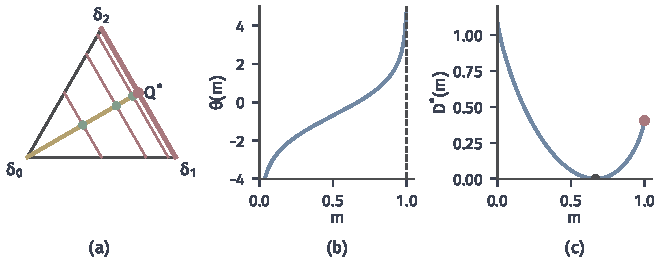
\includegraphics[width=112mm]{figures/07-probability/07-distribution-optimization/matplotlib/dsel-boundary-face/figure.pdf}
 \caption{边界上的矩，$T(x)=\mathbf{1}_{\{x\geq1\}}$，$P$均匀。(a)倾斜族是从$\delta_0$到$(0,\frac12,\frac12)$的线段（黄）；细红线是$m=0.5,0.8,0.95$的约束，绿点是各自的最优分布；粗红线是$m=1$时的可行集合，即$q(0)=0$的那条边，红点是最优分布。(b)参数$\theta(m)$，$m\to1$时发散。(c)最优值$D^{*}(m)$，在$m=2/3$处为零（$P$本身可行），在$m=1$处连续地达到$\ln\frac32$。}
 \label{fig:dsel-boundary-face}
\end{BookInlineFigure}

一般情形的结论如下。

\begin{theorem}[边界上的矩]
\label{thm:dsel-boundary}
设$\mathcal{X}$有限，$p(x)>0$对每个$x$成立，$\bm{m}\in\mathcal{M}\setminus\operatorname{ri}\mathcal{M}$。则
\begin{enumerate}
 \item 问题~\eqref{eq:dsel-min-kl-problem}有最优分布；
 \item 存在$\bm{a}\in\mathbb{R}^{k}$与$c\in\mathbb{R}$，使$\langle\bm{a},\bm{T}(x)\rangle\leq c$对一切$x$成立，$\langle\bm{a},\bm{m}\rangle=c$，且集合$F=\{x:\langle\bm{a},\bm{T}(x)\rangle=c\}$不是整个$\mathcal{X}$；每个$Q\in\mathcal{C}_{\bm{m}}$都满足$Q(F)=1$，因而没有任何$Q_{\bm{\theta}}$属于$\mathcal{C}_{\bm{m}}$；
 \item 对$Q(F)=1$的$Q$，记$P_F=P(\cdot\mid F)$，有
 \begin{equation}
 D_{\mathrm{KL}}(Q\Vert P)=D_{\mathrm{KL}}(Q\Vert P_F)-\ln P(F) ;
 \label{eq:dsel-face-reduction}
 \end{equation}
 \item 若$\bm{m}$属于$\operatorname{conv}\{\bm{T}(x):x\in F\}$的相对内部，则最优分布是$P_F$沿$\bm{T}$的倾斜$Q^{*}_F$，并且对满足$\mathbb{E}_{Q^{*}_F}[\bm{T}]=\bm{m}$的参数$\bm{\theta}_F$，$s\to+\infty$时$Q_{\bm{\theta}_F+s\bm{a}}\to Q^{*}_F$。
\end{enumerate}
\end{theorem}

\begin{proof}
第一部分。$\mathcal{C}_{\bm{m}}$由线性等式与非负性在概率单纯形中定出，是非空的有界闭集；$p>0$时$Q\mapsto\sum_xq(x)\ln(q(x)/p(x))$在单纯形上连续（约定$0\ln0=0$）。连续函数在非空紧集上取到最小值。

第二部分。$\mathcal{M}$是有限个点的凸包，$\bm{m}$在它的相对边界上。在仿射包$\operatorname{aff}\mathcal{M}$内对$\mathcal{M}$用凸集的支撑超平面定理，得到$\bm{a}\in L$（$L$是$\operatorname{aff}\mathcal{M}$的方向子空间）与$c$，使$\langle\bm{a},\bm{t}\rangle\leq c$对$\bm{t}\in\mathcal{M}$成立，$\langle\bm{a},\bm{m}\rangle=c$，且$\langle\bm{a},\cdot\rangle$在$\mathcal{M}$上不是常数。最后一点说明$F\neq\mathcal{X}$。对$Q\in\mathcal{C}_{\bm{m}}$，
\[
 \sum_xq(x)\bigl(c-\langle\bm{a},\bm{T}(x)\rangle\bigr)=c-\langle\bm{a},\bm{m}\rangle=0 .
\]
各项非负而和为零，所以$x\notin F$时$q(x)=0$，即$Q(F)=1$。每个$Q_{\bm{\theta}}$在所有状态上为正，不满足这一点。

第三部分。$x\in F$时$p_F(x)=p(x)/P(F)$，所以
\[
 \ln\frac{q(x)}{p(x)}=\ln\frac{q(x)}{p_F(x)}-\ln P(F) .
\]
乘以$q(x)$对$x\in F$求和，即得式~\eqref{eq:dsel-face-reduction}。所以在$F$上，原问题与以$P_F$为参考分布的同一问题只差常数$-\ln P(F)$。

第四部分。对状态集$F$、参考分布$P_F$与约束$\bm{m}$用定理~\ref{thm:dsel-min-kl}，得到最优分布$Q^{*}_F$与参数$\bm{\theta}_F$；由第三部分它也是原问题的最优分布。对$s>0$，
\[
 q_{\bm{\theta}_F+s\bm{a}}(x)\propto p(x)\,\mathrm{e}^{\langle\bm{\theta}_F,\bm{T}(x)\rangle}\,\mathrm{e}^{s(\langle\bm{a},\bm{T}(x)\rangle-c)} ,
\]
这里把各项同乘了与$x$无关的$\mathrm{e}^{-sc}$。$s\to\infty$时，最后一个因子在$F$上恒为$1$，在$F$外趋于$0$。归一化后的极限正比于$p(x)\mathrm{e}^{\langle\bm{\theta}_F,\bm{T}(x)\rangle}\mathbf{1}_F(x)$，这就是$Q^{*}_F$。
\end{proof}

若$\bm{m}$在$\operatorname{conv}\{\bm{T}(x):x\in F\}$中仍在相对边界上，对$F$重复第二、三部分，支持再缩小一次；状态有限，几步之内就会停下。在上面的例子中，$\bm{a}=1$，$c=1$，$F=\{1,2\}$，$T$在$F$上恒为$1$，$P_F=(0,\tfrac12,\tfrac12)$不需再倾斜，最优值$-\ln P(F)=\ln\tfrac32$。

边界情形说明了有限参数公式的局限。最优分布存在，也仍是某个倾斜的极限，但它收缩了支持，不能写成任何有限$\bm{\theta}$的$Q_{\bm{\theta}}$。数值上，Newton迭代的$\bm{\theta}$会越走越远：在$T(x)=x$、$m=2$的例子中，参数每步大约增加$1$，残差每步只缩小到约$1/\mathrm{e}$，内部情形的二次收敛不复存在。遇到这种迹象，应当先识别哪些状态的概率必须为零，在缩小后的状态集上重新求解，而不是继续追逐发散的参数。对偶函数的上确界仍等于最优值，沿$\bm{\theta}_F+s\bm{a}$可以逼近，只是取不到。
